%%%%%%%%%%%%%%%%%%%%%%%%%%%%%%%%%%%%%%%%%%%%%%%%%%%%%%%%%%%%%%%%%%%%%%
%%%%%%%%%%%%%%%%%%%%%%%%%%%%%%%%%%%%%%%%%%%%%%%%%%%%%%%%%%%%%%%%%%%%%%
%%
%% IVT LaTeX template
%%   Kirill M�ller
%%   kirill.mueller@ivt.baug.ethz.ch
%%
%%%%%%%%%%%%%%%%%%%%%%%%%%%%%%%%%%%%%%%%%%%%%%%%%%%%%%%%%%%%%%%%%%%%%%
%%%%%%%%%%%%%%%%%%%%%%%%%%%%%%%%%%%%%%%%%%%%%%%%%%%%%%%%%%%%%%%%%%%%%%

%%%%%%%%%%%%%%%%%%%%%%%%%%%%%%%%%%%%%%%%%%%%%%%%%%%%%%%%%%%%%%%%%%%%%%
%%%%%%%%%%%%%%%%%%%%%%%%%%%%%%%%%%%%%%%%%%%%%%%%%%%%%%%%%%%%%%%%%%%%%%
%%
%% Encoding check:
%%   �  �  �  �  �  �  �  �  �  �  �  �  �  �  �  �  �  �  �  �  �  �
%%
%%   If the above contains rubbish, please re-open this file using
%%   one of the following encodings: Latin1, ISO-8859-1, Windows-1252.
%%   DO NOT save the file in this case!
%%
%%%%%%%%%%%%%%%%%%%%%%%%%%%%%%%%%%%%%%%%%%%%%%%%%%%%%%%%%%%%%%%%%%%%%%
%%%%%%%%%%%%%%%%%%%%%%%%%%%%%%%%%%%%%%%%%%%%%%%%%%%%%%%%%%%%%%%%%%%%%%

%%%%%%%%%%%%%%%%%%%%%%%%%%%%%%%%%%%%%%%%%%%%%%%%%%%%%%%%%%%%%%%%%%%%%%
%%%%%%%%%%%%%%%%%%%%%%%%%%%%%%%%%%%%%%%%%%%%%%%%%%%%%%%%%%%%%%%%%%%%%%
%%
%% This is an example for writing a paper at the IVT.
%% It supports English and German language.
%% By using it, it is possible to switch paper layouts easily
%% (e.g., working paper style into TRB style)
%%
%% The easiest way to write you own paper is to create an
%% appropriate directory stucture in the papers subdirectory
%% i.e. papers/strc/2007/mypaper,
%% copy this template and modify it there.
%%
%% See the note below on renaming the main file.
%%
%% Each keyword is documented. Just follow the instructions...
%% Enjoy!
%%
%%%%%%%%%%%%%%%%%%%%%%%%%%%%%%%%%%%%%%%%%%%%%%%%%%%%%%%%%%%%%%%%%%%%%%
%%%%%%%%%%%%%%%%%%%%%%%%%%%%%%%%%%%%%%%%%%%%%%%%%%%%%%%%%%%%%%%%%%%%%%

%%%%%%%%%%%%%%%%%%%%%%%%%%%%%%%%%%%%%%%%%%%%%%%%%%%%%%%%%%%%%%%%%%%%%%
%%%%%%%%%%%%%%%%%%%%%%%%%%%%%%%%%%%%%%%%%%%%%%%%%%%%%%%%%%%%%%%%%%%%%%
%%
%% IMPORTANT NOTE ON FILE RENAMES:
%%   If you rename this file, look for the text "Template"
%%   in all files and change this to the new filename, too.
%%   In Linux/Mac OS X/Windows+cygwin: Execute the following command
%%     in the template directory (substitute NewName by the new
%%     base of the new file name):
%%
%%     find -maxdepth 1 -type f -exec sed -i 's/[T]emplate/NewName/g' \{\} \+
%%     mmv 'T''emplate.*' 'NewName.#1'
%%
%%   In Windows (vanilla): Use your favorite find-in-text-files tool
%%
%%%%%%%%%%%%%%%%%%%%%%%%%%%%%%%%%%%%%%%%%%%%%%%%%%%%%%%%%%%%%%%%%%%%%%
%%%%%%%%%%%%%%%%%%%%%%%%%%%%%%%%%%%%%%%%%%%%%%%%%%%%%%%%%%%%%%%%%%%%%%

%%%%%%%%%%%%%%%%%%%%%%%%%%%%%%%%%%%%%%%%%%%%%%%%%%%%%%%%%%%%%%%%%%%%%%
%% Location of the common files
%%   If unsure, please leave this as it is
\newcommand{\mypath}{_latexfiles/}
%\newcommand{\mypath}{../../../}
%%%%%%%%%%%%%%%%%%%%%%%%%%%%%%%%%%%%%%%%%%%%%%%%%%%%%%%%%%%%%%%%%%%%%%

%%%%%%%%%%%%%%%%%%%%%%%%%%%%%%%%%%%%%%%%%%%%%%%%%%%%%%%%%%%%%%%%%%%%%%
%% language specification:
%%   Here you define in which langugage your paper will be written.
%%   There are ALWAYS 2 languages to define (even you do not need it.)
%%   Since we are writing only in German or English, other languages
%%   are not supported.
%%   Choose either 'german' or 'english' as your first language.
\newcommand{\myfirstlang}{english}
%%%%%%%%%%%%%%%%%%%%%%%%%%%%%%%%%%%%%%%%%%%%%%%%%%%%%%%%%%%%%%%%%%%%%%

%%%%%%%%%%%%%%%%%%%%%%%%%%%%%%%%%%%%%%%%%%%%%%%%%%%%%%%%%%%%%%%%%%%%%%
%% Include Paper-Layout:
%%   Here the ivt working paper layout is chosen
%%   For changing this paper into i.e. TRB layout just change "ivt-wp"
%%   to "trb"
\input{\mypath_layouts/strc}
%%%%%%%%%%%%%%%%%%%%%%%%%%%%%%%%%%%%%%%%%%%%%%%%%%%%%%%%%%%%%%%%%%%%%%

%%%%%%%%%%%%%%%%%%%%%%%%%%%%%%%%%%%%%%%%%%%%%%%%%%%%%%%%%%%%%%%%%%%%%%
%%%%%%%%%%%%%%%%%%%%%%%%%%%%%%%%%%%%%%%%%%%%%%%%%%%%%%%%%%%%%%%%%%%%%%
%%
%% START DOCUMENT KEYWORDS
%%   In this part you can define Authors, Date, Titlefigure, etc...
%%
%%%%%%%%%%%%%%%%%%%%%%%%%%%%%%%%%%%%%%%%%%%%%%%%%%%%%%%%%%%%%%%%%%%%%%
%%%%%%%%%%%%%%%%%%%%%%%%%%%%%%%%%%%%%%%%%%%%%%%%%%%%%%%%%%%%%%%%%%%%%%

%%%%%%%%%%%%%%%%%%%%%%%%%%%%%%%%%%%%%%%%%%%%%%%%%%%%%%%%%%%%%%%%%%%%%%
%% The figure to include in the title page:
%% - {path/to/the/figure}: includes this figure in the title
%% - {}: no figure will be included
%% Note:
%%   do not write the ending of your figure ("MATSimLoop" instead
%%   of "MATSimLoop.pdf")
\newcommand{\mytitlefigure}{}
%%%%%%%%%%%%%%%%%%%%%%%%%%%%%%%%%%%%%%%%%%%%%%%%%%%%%%%%%%%%%%%%%%%%%%

%%%%%%%%%%%%%%%%%%%%%%%%%%%%%%%%%%%%%%%%%%%%%%%%%%%%%%%%%%%%%%%%%%%%%%
%% The title of the paper
\newcommand{\mytitle}{Estimating externalities from GPS traces using MATSim}
%%%%%%%%%%%%%%%%%%%%%%%%%%%%%%%%%%%%%%%%%%%%%%%%%%%%%%%%%%%%%%%%%%%%%%

%%%%%%%%%%%%%%%%%%%%%%%%%%%%%%%%%%%%%%%%%%%%%%%%%%%%%%%%%%%%%%%%%%%%%%
%% The institution (group) for which the paper is written
\newcommand{\myinstitutionDE}{}
\newcommand{\myinstitutionEN}{IVT ETHZ}
%%%%%%%%%%%%%%%%%%%%%%%%%%%%%%%%%%%%%%%%%%%%%%%%%%%%%%%%%%%%%%%%%%%%%%

%%%%%%%%%%%%%%%%%%%%%%%%%%%%%%%%%%%%%%%%%%%%%%%%%%%%%%%%%%%%%%%%%%%%%%
%% The number of the paper
\newcommand{\mynumber}{8XX}
%%%%%%%%%%%%%%%%%%%%%%%%%%%%%%%%%%%%%%%%%%%%%%%%%%%%%%%%%%%%%%%%%%%%%%

%%%%%%%%%%%%%%%%%%%%%%%%%%%%%%%%%%%%%%%%%%%%%%%%%%%%%%%%%%%%%%%%%%%%%%
%% The year of the paper
\newcommand{\myyear}{2018}
%%%%%%%%%%%%%%%%%%%%%%%%%%%%%%%%%%%%%%%%%%%%%%%%%%%%%%%%%%%%%%%%%%%%%%

%%%%%%%%%%%%%%%%%%%%%%%%%%%%%%%%%%%%%%%%%%%%%%%%%%%%%%%%%%%%%%%%%%%%%%
%% The month of the paper
%% - include only: jan,feb,mar,apr,may,jun,jul,aug,sep,oct,nov,dec
\newcommand{\mymonth}{may}
%%%%%%%%%%%%%%%%%%%%%%%%%%%%%%%%%%%%%%%%%%%%%%%%%%%%%%%%%%%%%%%%%%%%%%

%%%%%%%%%%%%%%%%%%%%%%%%%%%%%%%%%%%%%%%%%%%%%%%%%%%%%%%%%%%%%%%%%%%%%%
%% The day of the paper
%% - include day in number 1,..., 12,..., 31
\newcommand{\myday}{01}
%%%%%%%%%%%%%%%%%%%%%%%%%%%%%%%%%%%%%%%%%%%%%%%%%%%%%%%%%%%%%%%%%%%%%%

%%%%%%%%%%%%%%%%%%%%%%%%%%%%%%%%%%%%%%%%%%%%%%%%%%%%%%%%%%%%%%%%%%%%%%
%%
%% Define the authors
%% - if author name is left empty
%%   \newcommand{\mysecondauthor}{}
%%   it is not shown
%% - keep the right order (first, second, etc...) and keep the
%%   remaining entries empty!
%% - also add the way the authors appear in the reference style
%%
%%%%%%%%%%%%%%%%%%%%%%%%%%%%%%%%%%%%%%%%%%%%%%%%%%%%%%%%%%%%%%%%%%%%%%

%%%%%%%%%%%%%%%%%%%%%%%%%%%%%%%%%%%%%%%%%%%%%%%%%%%%%%%%%%%%%%%%%%%%%%
%% The author 1
\newcommand{\myfirstauthor}{Christopher Tchervenkov}
\newcommand{\myfirstauthorREF}{Tchervenkov,~C.}
%%%%%%%%%%%%%%%%%%%%%%%%%%%%%%%%%%%%%%%%%%%%%%%%%%%%%%%%%%%%%%%%%%%%%%
%% The author 2
\newcommand{\mysecondauthor}{Joseph Molloy}
\newcommand{\mysecondauthorREF}{Molloy,~J}
%%%%%%%%%%%%%%%%%%%%%%%%%%%%%%%%%%%%%%%%%%%%%%%%%%%%%%%%%%%%%%%%%%%%%%
%% The author 3
\newcommand{\mythirdauthor}{Kay W. Axhausen}
\newcommand{\mythirdauthorREF}{Axhausen,~K.W.}
%%%%%%%%%%%%%%%%%%%%%%%%%%%%%%%%%%%%%%%%%%%%%%%%%%%%%%%%%%%%%%%%%%%%%%
%% The author 4
\newcommand{\myfourthauthor}{}
\newcommand{\myfourthauthorREF}{}
%%%%%%%%%%%%%%%%%%%%%%%%%%%%%%%%%%%%%%%%%%%%%%%%%%%%%%%%%%%%%%%%%%%%%%
%% The author 5
\newcommand{\myfifthauthor}{}
\newcommand{\myfifthauthorREF}{}
%%%%%%%%%%%%%%%%%%%%%%%%%%%%%%%%%%%%%%%%%%%%%%%%%%%%%%%%%%%%%%%%%%%%%%
%% The author 6
\newcommand{\mysixthauthor}{}
\newcommand{\mysixthauthorREF}{}
%%%%%%%%%%%%%%%%%%%%%%%%%%%%%%%%%%%%%%%%%%%%%%%%%%%%%%%%%%%%%%%%%%%%%%
%% .. up to 12 authors supported by the templates
%%%%%%%%%%%%%%%%%%%%%%%%%%%%%%%%%%%%%%%%%%%%%%%%%%%%%%%%%%%%%%%%%%%%%%

%%%%%%%%%%%%%%%%%%%%%%%%%%%%%%%%%%%%%%%%%%%%%%%%%%%%%%%%%%%%%%%%%%%%%%
%%
%% Define the addresses
%% - if author name is left empty
%%   \newcommand{\mysecondaddress}{}
%%   it is not shown
%% - if two authors share the same affiliation, they should also use
%%   the same address
%% - keep the right order (first, second, etc...) and keep the
%%   remaining entries empty!
%% - also add the way the authors appear in the reference style
%%
%%%%%%%%%%%%%%%%%%%%%%%%%%%%%%%%%%%%%%%%%%%%%%%%%%%%%%%%%%%%%%%%%%%%%%

%%%%%%%%%%%%%%%%%%%%%%%%%%%%%%%%%%%%%%%%%%%%%%%%%%%%%%%%%%%%%%%%%%%%%%
%% Increase this if you have more than two addresses
\newcommand{\mynumaddresscolumns}{2}
%%%%%%%%%%%%%%%%%%%%%%%%%%%%%%%%%%%%%%%%%%%%%%%%%%%%%%%%%%%%%%%%%%%%%%
%% The first address
\newcommand{\myfirstaddress}{
  \createcontact{\myfirstauthor}%
  {IVT}
  {ETHZ}
  {CH-8093 Z�rich}
  {+41 44 633 33 17}
  {}
  {christopher.tchervenkov@ivt.baug.ethz.ch}
}
%%%%%%%%%%%%%%%%%%%%%%%%%%%%%%%%%%%%%%%%%%%%%%%%%%%%%%%%%%%%%%%%%%%%%%
%% The second address
\newcommand{\mysecondaddress}{
  \createcontact{\mysecondauthor}%
  {IVT}
  {ETHZ}
  {CH-8093 Z�rich}
  {+41 44 633 31 51}
  {}
  {joseph.molloy@ivt.baug.ethz.ch}
}
%%%%%%%%%%%%%%%%%%%%%%%%%%%%%%%%%%%%%%%%%%%%%%%%%%%%%%%%%%%%%%%%%%%%%%
%% The third address
\newcommand{\mythirdaddress}{
  \createcontact{\mythirdauthor}%
  {IVT}
  {ETHZ}
  {CH-8093 Z�rich}
  {+41 44 633 39 43}
  {}
  {axhausen@ivt.baug.ethz.ch}
}
%%%%%%%%%%%%%%%%%%%%%%%%%%%%%%%%%%%%%%%%%%%%%%%%%%%%%%%%%%%%%%%%%%%%%%
%% The fourth address
\newcommand{\myfourthaddress}{%
}
%%%%%%%%%%%%%%%%%%%%%%%%%%%%%%%%%%%%%%%%%%%%%%%%%%%%%%%%%%%%%%%%%%%%%%
%% The fifth address
\newcommand{\myfifthaddress}{%
}
%%%%%%%%%%%%%%%%%%%%%%%%%%%%%%%%%%%%%%%%%%%%%%%%%%%%%%%%%%%%%%%%%%%%%%
%% The sixth address
\newcommand{\mysixthaddress}{%
}

%%%%%%%%%%%%%%%%%%%%%%%%%%%%%%%%%%%%%%%%%%%%%%%%%%%%%%%%%%%%%%%%%%%%%%
%% The keywords (English)
\newcommand{\mykeywordsEN}{Keywords, in English, language}
%%%%%%%%%%%%%%%%%%%%%%%%%%%%%%%%%%%%%%%%%%%%%%%%%%%%%%%%%%%%%%%%%%%%%%

%%%%%%%%%%%%%%%%%%%%%%%%%%%%%%%%%%%%%%%%%%%%%%%%%%%%%%%%%%%%%%%%%%%%%%
%% The keywords (German)
\newcommand{\mykeywordsDE}{Schl�sselw�rter, auf Deutsch, Sprache}
%%%%%%%%%%%%%%%%%%%%%%%%%%%%%%%%%%%%%%%%%%%%%%%%%%%%%%%%%%%%%%%%%%%%%%

%%%%%%%%%%%%%%%%%%%%%%%%%%%%%%%%%%%%%%%%%%%%%%%%%%%%%%%%%%%%%%%%%%%%%%
%%%%%%%%%%%%%%%%%%%%%%%%%%%%%%%%%%%%%%%%%%%%%%%%%%%%%%%%%%%%%%%%%%%%%%
%%
%% END DOCUMENT KEYWORDS
%%
%%%%%%%%%%%%%%%%%%%%%%%%%%%%%%%%%%%%%%%%%%%%%%%%%%%%%%%%%%%%%%%%%%%%%%
%%%%%%%%%%%%%%%%%%%%%%%%%%%%%%%%%%%%%%%%%%%%%%%%%%%%%%%%%%%%%%%%%%%%%%


%%%%%%%%%%%%%%%%%%%%%%%%%%%%%%%%%%%%%%%%%%%%%%%%%%%%%%%%%%%%%%%%%%%%%%
%%%%%%%%%%%%%%%%%%%%%%%%%%%%%%%%%%%%%%%%%%%%%%%%%%%%%%%%%%%%%%%%%%%%%%
%%
%% START USER DEFINED COMMANDS
%%   Sometimes latex does not do hyphenations. This happens if it
%%   does not recognize a specific word. with "\hyphenation"
%%   you can add rules for those words
%% for advanced users:
%%   Advanced users can add additional commands here
%%
%%%%%%%%%%%%%%%%%%%%%%%%%%%%%%%%%%%%%%%%%%%%%%%%%%%%%%%%%%%%%%%%%%%%%%
%%%%%%%%%%%%%%%%%%%%%%%%%%%%%%%%%%%%%%%%%%%%%%%%%%%%%%%%%%%%%%%%%%%%%%

%%%%%%%%%%%%%%%%%%%%%%%%%%%%%%%%%%%%%%%%%%%%%%%%%%%%%%%%%%%%%%%%%%%%%%
%% Word split: unknown words for latex. show how to split them.
\hyphenation{Trenn-re-geln}
%%%%%%%%%%%%%%%%%%%%%%%%%%%%%%%%%%%%%%%%%%%%%%%%%%%%%%%%%%%%%%%%%%%%%%
\newcommand{\red}[1]{\textcolor{red}{#1}}

%%%%%%%%%%%%%%%%%%%%%%%%%%%%%%%%%%%%%%%%%%%%%%%%%%%%%%%%%%%%%%%%%%%%%%
%%%%%%%%%%%%%%%%%%%%%%%%%%%%%%%%%%%%%%%%%%%%%%%%%%%%%%%%%%%%%%%%%%%%%%
%%
%% END USER DEFINED COMMANDS
%%
%%%%%%%%%%%%%%%%%%%%%%%%%%%%%%%%%%%%%%%%%%%%%%%%%%%%%%%%%%%%%%%%%%%%%%
%%%%%%%%%%%%%%%%%%%%%%%%%%%%%%%%%%%%%%%%%%%%%%%%%%%%%%%%%%%%%%%%%%%%%%

%%%%%%%%%%%%%%%%%%%%%%%%%%%%%%%%%%%%%%%%%%%%%%%%%%%%%%%%%%%%%%%%%%%%%%
%%%%%%%%%%%%%%%%%%%%%%%%%%%%%%%%%%%%%%%%%%%%%%%%%%%%%%%%%%%%%%%%%%%%%%
%%
%% To speed up compilation, you can split this file and move the
%%   contents of the upper part (just before the %&Template line)
%%   to a new file named Template.ltx.  This requires a working
%%   installation of GNU Make (included in Linux/Mac OS X,
%%   in Windows: through cygwin or GnuWin32).
%%
%&Template

%%%%%%%%%%%%%%%%%%%%%%%%%%%%%%%%%%%%%%%%%%%%%%%%%%%%%%%%%%%%%%%%%%%%%%
%%%%%%%%%%%%%%%%%%%%%%%%%%%%%%%%%%%%%%%%%%%%%%%%%%%%%%%%%%%%%%%%%%%%%%
%%
%% START OF DOCUMENT
%%   Here actually begins your document. The things below
%%   are a typical order in which a paper should be organized.
%%   Sometimes, editors have other suggestions. In this case
%%   just change the order in which each part should appear.
%%
%%%%%%%%%%%%%%%%%%%%%%%%%%%%%%%%%%%%%%%%%%%%%%%%%%%%%%%%%%%%%%%%%%%%%%
%%%%%%%%%%%%%%%%%%%%%%%%%%%%%%%%%%%%%%%%%%%%%%%%%%%%%%%%%%%%%%%%%%%%%%

\usepackage{multicol}


\begin{document}

%%%%%%%%%%%%%%%%%%%%%%%%%%%%%%%%%%%%%%%%%%%%%%%%%%%%%%%%%%%%%%%%%%%%%%
%% Include the title page
\createtitlepage
%%%%%%%%%%%%%%%%%%%%%%%%%%%%%%%%%%%%%%%%%%%%%%%%%%%%%%%%%%%%%%%%%%%%%%

%%%%%%%%%%%%%%%%%%%%%%%%%%%%%%%%%%%%%%%%%%%%%%%%%%%%%%%%%%%%%%%%%%%%%%
%% Page numbering is taken care of by the templates
%%%%%%%%%%%%%%%%%%%%%%%%%%%%%%%%%%%%%%%%%%%%%%%%%%%%%%%%%%%%%%%%%%%%%%

%%%%%%%%%%%%%%%%%%%%%%%%%%%%%%%%%%%%%%%%%%%%%%%%%%%%%%%%%%%%%%%%%%%%%%
%% Table of contents
%\tableofcontents
%%%%%%%%%%%%%%%%%%%%%%%%%%%%%%%%%%%%%%%%%%%%%%%%%%%%%%%%%%%%%%%%%%%%%%

%%%%%%%%%%%%%%%%%%%%%%%%%%%%%%%%%%%%%%%%%%%%%%%%%%%%%%%%%%%%%%%%%%%%%%
%% List of figures and tables
%\listoffigures
%%%%%%%%%%%%%%%%%%%%%%%%%%%%%%%%%%%%%%%%%%%%%%%%%%%%%%%%%%%%%%%%%%%%%%

%%%%%%%%%%%%%%%%%%%%%%%%%%%%%%%%%%%%%%%%%%%%%%%%%%%%%%%%%%%%%%%%%%%%%%
%% List of tables
%\listoftables
%%%%%%%%%%%%%%%%%%%%%%%%%%%%%%%%%%%%%%%%%%%%%%%%%%%%%%%%%%%%%%%%%%%%%%

%%%%%%%%%%%%%%%%%%%%%%%%%%%%%%%%%%%%%%%%%%%%%%%%%%%%%%%%%%%%%%%%%%%%%%
%% If the next part should start at a new page insert \clearpage
%% command
\clearpage
%%%%%%%%%%%%%%%%%%%%%%%%%%%%%%%%%%%%%%%%%%%%%%%%%%%%%%%%%%%%%%%%%%%%%%

%%%%%%%%%%%%%%%%%%%%%%%%%%%%%%%%%%%%%%%%%%%%%%%%%%%%%%%%%%%%%%%%%%%%%%
%% Page numbering is taken care of by the templates
%%%%%%%%%%%%%%%%%%%%%%%%%%%%%%%%%%%%%%%%%%%%%%%%%%%%%%%%%%%%%%%%%%%%%%

%%%%%%%%%%%%%%%%%%%%%%%%%%%%%%%%%%%%%%%%%%%%%%%%%%%%%%%%%%%%%%%%%%%%%%

%%%%%%%%%%%%%%%%%%%%%%%%%%%%%%%%%%%%%%%%%%%%%%%%%%%%%%%%%%%%%%%%%%%%%%
%% ABSTRACT (first language)
%%   You can write it just here, if you want. You can also include
%%   an external .tex file (for better organization of you paper)
%%   The abstract MUST always be embedded into a command:
%%     \createabstract{
%%     This is an
%%     example abstract.
%%     }
%%   Be sure that your abstract is embedded into the curly brackets.
%%
%%   You can also put the abstract in a seperate .tex file for better
%%   organization. The command then is:
%%     \input{abstract-first}
%%   see also below (include sections)
\createabstract{Providing people with information on the external costs of their mobility, including generated emissions, contribution to congestion, and noise pollution, has been shown to influence their travel behavior.
However, directly measuring these externalities at the source is unfeasible.
We have therefore developed a pipeline for estimating the generated externalities of recorded trips using the multi-agent simulation software MATSim. First, collected GPS traces are matched to the MATSim network and converted to MATSim events.
These events are then processed to impute externalities for each individual.
Emission values for various pollutants are calculated for each link using  the HBEFA database, accounting for vehicle type, road category and traffic conditions.
For congestion, we leverage MATSim modules developed by Kaddoura to compute average link delays for each hour of the day using the MATSim scenario of Switzerland, which are then assigned to links traveled by the participants.
We adapt this pipeline to further account for the Swiss valuation of externalities.
To validate our approach, the externalities generated for the Swiss MATSim scenario will be compared to ARE estimates and the swiss norm values.
The application of the pipeline will be demonstrated for GPS traces collected from the SBB Green Class project.
}
\section{Introduction}

It is increasingly recognized that both the environmental and social costs of travel need to be internalized to meet the demand on already strained transport networks by encouraging shifts in travel patterns. 
In this direction, there is a growing body of evidence that informal feedback on energy use can encourage more efficient behavior, both regarding home energy use \citep{faruqui2010impact} and travel behavior \citep{taniguchi2003psychological, fujii2006determinants}.
However, providing feedback on external costs in transport is particularly challenging, due to the heterogeneous nature of the users and privacy constraints.

%%Start here on externalities - Joe, already written
The main externalities of transportation can be divided into two groups: Those that affect other road users, namely congestion, and those that affect non-road users such as noise and emissions \cite{button2004rationale}.
The impact of congestion is primarily the loss of time spent waiting in traffic, where as emissions and noise have both environmental and health consequences.
When a person chooses to drive on a road, they only have to pay for the private time and car usage costs.
However, they do not have to pay the \textit{marginal social cost} (MSC) of their trip.
That is, the additional costs the driver imposes on other drivers by increasing demand on the route.
From economic theory, internalising this MSC in the form of a tax would reduce congestion and provide an overall social benefit \cite{arnott1994economics, pigou2013economics}). 

Micrsosimulation provides advantages from both the supply (network representation) and demand (individual agents) sides when modeling road pricing.
\citet{arnott2001economic} notes that traditional macroscopic models focus on link congestion, while ignoring or simplifying other elements of congestion such as nodal congestion, parking and interactions with pedestrians and spillback.
Microsimulated models allow for the representation of non-homogenous driver behaviour and preferences.
In particular, the importance of value of time heterogenity among individuals in road pricing models has been recognised by numerous researchers \citet{small2001value, verhoef2004product}.
Modern traffic microsimulation frameworks such as MATSim \cite{balmer2009matsim} are to capture range of externalities.

\citet{kaddoura2015marginal} developed an agent based marginal cost-pricing approaches for congestion, emissions and noise exteralities, and applied numerous models successfully to a large scale scenario of Greater Berlin.
When considering the internalisation of congestion costs, a particular contribution of his work, was to assign the external congestion costs to the causing agents.
In particular, \citet{kaddoura2015marginal} notes that it is simple to calculate the incurred congestion for each agent, but much more challenging to map it back to the causing agent.
The approach calculates each agent's contribution to the delays on traveled links using a queue based node-link model including spillback.

In real networks such an approach requires knowing the location and VTTS of every driver connected to a particular incident of congestion.
This is clearly unrealistic. Instead, this work presents an approach to impute externalities using just the GPS trace of the trip, a representation of the road network and aggregated congestion values generated from an agent-based MATSim simulation for Switzerland.

\subsection{Swiss MATSim Scenario}
%%Chris or Joe
The IVT 2015 Baseline Scenario \cite{boesch2015ivt} represents a typical working day in Switzerland for the year 2015.
As a MATSim scenario, the population consists of individual agents, each with daily travel plans (preferences) and social-demographic characteristics.
These agents represent the entire population of Switzerland on the network from \cite{boesch2015network}.
The 2015 scenario extends the work of \cite{Balmer2007switzerland} to add households and household incomes and model elements. The scenario is available in 1\%, 10\% and 100\% samples with respectively increasing runtimes. 

\subsection{Analysis of road transport externalities in Switzerland}  %%%Swiss norms, ARE report, HBEFA}

Numerous sources are available for the analysis of external costs in Switzerland, including Standards, government reports and databases. These sources guide and inform the evaluation of new and existing infrastructure projects. A report on the external costs and benefits analysis of transport in Switzerland is available from the \citet{are2016externalcosts}, built on the methodology developed in \cite{ecoplaninfras2014externeeffekte}.
It presents the most recent external cost-benefit analysis for the Swiss transport system, primarily focusing on external environmental, health and accident-related costs.
Specifically, external costs for 12 different cost categories are computed, differentiated according to three different perspectives: transport mode (road/rail/air/water, passenger/freight, vehicle type), transport type (particulary heavy vehicles) and transport user. 

For the modeling of road transport pollutant emissions in Switzerland (and other European countries), emission factors are generally taken from the Handbook for Emission Factor Analysis (HBEFA) \cite{maibach2008emissions}.
The HBEFA database contains emission factors for a range vehicle categories and traffic situations, differentiated by emission type, pollutant and year. The HBEFA is the standard for road pollutant analysis in Germany, Switzerland and Austria, and is supported by the European Comission. 

\citet{foen2010pollutants} use the HBEFA to provide an detailed analysis of past and predicted future pollutant emissions, covering road transport in Switzerland from 1990 to 2035.
Emissions values are calculated for three emissions types: emissions when engine is in hot operating condition, cold-start emissions and evaporation emissions.
The calculation of these values require both traffic volume data as well as the emissions factors from the HBEFA for each emission type.
The authors model the development of the vehicle fleet composition, vehicle specific mileage and emission standards trends, resulting 
traffic volumes (mileage and start/stop processes) differentiated by vehicle category, emission standard and road category.
These traffic volumes are then multiplied by the corresponding emissions factors to obtain the final emissions values.

Concerning congestion specifically, \cite{mkinfras2016staukosten} estimate the external traffic delay costs for the years 2009 to 2014.
The objective of this study was to estimate vehicle hours of delay and identify the contribution from heavy vehicles.
For 2013, this was achieved by combining and aligning INRIX traffic flow data and traffic demand data from the National Passenger Transport Model.
The time lost per road section was calculated by subtracting the free-flow travel time from actual travel time, where traffic jams are considered to occur only when the actual speed is less than 65\% of the free-flow speed.
For the other years, online data from the Federal Roads Office (FEDRO) counting stations was used.
A summary of their results is provided in \Cref{tab:vehHoursDelayMkInfras}.
The values provide a useful estimate of delay costs in Switzerland, however, the use of an "at-least" approach will tend to underestimate the lost time and resulting associated delay costs \cite{2016staukosten}.
%This is particularly the case for non-motorways road segments, where long road lengths, flawed speed data and lack of zero mean speed cases play a significant role.

\createtable%
{Updated estimated vehicle hours of delay for 2009-2014}%
{Updated estimates of vehicle hours of delay for 2009-2014 and comparison to previously reported values from ARE 2012 for Light (LMV) and Heavy Motorized Vehicles (HMV)}%
{\label{tab:vehHoursDelayMkInfras}}%
{%
  \begin{tabular}[c]{lrrrrrrrr}
    \toprule
    \multirow{3}{*}{} & & \multicolumn{7}{c}{Vehicle hours of delay (Mio/a)}\\ 
    & & \multicolumn{2}{c}{Motorway} & \multicolumn{2}{c}{Non-motorway} & \multicolumn{3}{c}{All roads}\\
    & &  LMV & HMV & LMV & HMV & LMV & HMV & Both\\
    \midrule
    \multirow{6}{*}{Updated}
    & 2009 & 11.41 & 0.53 & 11.23 & 0.22 & 22.64 & 0.75 & 23.39 \\
    & 2010 & 15.19 & 0.79 & 11.23 & 0.22 & 26.42 & 1.00 & 27.42 \\
    & 2011 & 15.68 & 0.81 & 11.23 & 0.22 & 26.90 & 1.03 & 27.93 \\
    & 2012 & 16.45 & 0.85 & 11.23 & 0.22 & 27.68 & 1.07 & 28.75 \\
    & 2013 & 15.67 & 0.82 & 11.23 & 0.22 & 26.90 & 1.04 & 27.93 \\
    & 2014 & 16.62 & 0.87 & 11.23 & 0.22 & 27.85 & 1.09 & 28.94 \\
    \midrule
    Previous & 2009 & 12.40 & 1.08 & 14.10 & 0.28 & 26.5 & 1.4 & 27.9 \\
    \bottomrule
  \end{tabular}
}%
{\cite{mkinfras2016staukosten}, p.141, Annexe A4}

The Swiss Association of Road and Transportation Experts (VSS) has published a series of norms (SN 641 82* : Cost Benefit Analysis
for Road Traffic) aimed at guiding the accessment of monetary effects and the cost benefit analysis of transport projects, policies and regulations.
Norms SN 641 820 (Basic Standard), SN 641 822a (Travel Time Costs for Passenger Traffic) and SN 641 828 (External Costs) can be of particular interest in the context of external cost evaluation.
For example, they provide standard values for time costs and willingness to pay per vehicle type and trip purposes as well as standard methods for evaluating the monetary impacts of air pollution and climate impacts.
 

\subsection{Green Class Data}
%%Joe
In the Green Class 2016 pilot project, the SBB created a new mobility offering for subscribers which consisted of a General Abonnenment (GA), an electric BMW i3, park+ride subscription, car and bike sharing subscriptions.
The 139 participants were tracked for the duration of the project using a mobile app enabled with GPS.

\red{how much detail on the work from geoINFK?} These GPS traces were processed to identify individual trips and modes of travel \cite{rabaul2016greenclassprocessing}.

The trip records contain the following information:
\begin{itemize}
  \item user id
  \item trip id
  \item start timestamp
  \item end timestamp
  \item identified mode of travel
\end{itemize}

Each GPS waypoint records contains: 
\begin{itemize}
  \item longitude
  \item latitude
  \item timestamp
  \item accuracy (meters)
  \item user id
\end{itemize}

\red {summary of trips, waypoints in table}

In total, for the 139 participants, there were 163,417 trips recorded, with an an average of 4 trips per person per day (see Table \ref{Table:green_class}). For this research, the dataset was filtered to only include those trips with either a personal car or the provided electric vehicle. This left  
Figure \ref{figure:waypoint_dist} presents the distribution of the number of gps points per trip. 
A large number of GPS points is important for accurate route detection and identification of the link entry and exit timings.

\createtable%
{Green Class Trips and Waypoints}%
{Green Class Trips and Waypoints}%
{\label{tab:green_class_gps_summary}}%
{%
\begin{tabular}{ l | r r | r r r}
                    & \multicolumn{2}{c|}{Full Dataset}  & \multicolumn{3}{c}{Within Switzerland}  \\ 
 
                    & Full Dataset  &   (E)cars & (E)cars   & Cars & E-cars \\ 
\hline
 Users            & \multicolumn{2}{c|}{139} & \multicolumn{3}{c}{139} \\  
 Trips            & 163,417       & 90,568    & 81,365    & 51,843    & 31,219\\  
 Trip Legs        & 163,417       & 100,865   & 90,040    & 57,426    & 32,614\\  
 GPS Points       &  152,813,375  &   30,285,999     &    19,931,558    & 10,915,620 & 9,015,938 \\ 
 GPS Points / Trip Leg &  935.11   &    302.30    &  224.51     &   193.5   &  278.56  \\  
 Trips/person/day & 4.97          & 3.05      & 2.94      & 2.94      & 2.94 \\  
\end{tabular}
}
{}

For this analysis, the dataset was filtered to include only trips with a start and finish within Switzerland using either the electric car or personal automobile. 



\section{Methodology}
%% i.e. Pipeline structure
%%Joe

% Pipeline for processing of GPS traces
%  - filtering of waypoints
%  - map matching using graphhopper
%  - remove matched trips that have an average speed over 120kmh, or a duration less than 1 minute - 9\% of trips removed.
%  - calculate link entry and exit times - simple formula
%  - convert to matsim events
%  - run traces through event processing to calculate externalities
%  	- for emissions cap link average speed at link freespeed 
%  	- road types taken from OSM
%  	- end result is calculation of emissions and delays for each trip leg
In this section, the methodology for imputing externalities on GPS is presented. For the imputation, reference values for air pollutant and congestion production are required. For emissions, the HEBFA database v3.2 is used. 
For congestion, the output of a 10\% sample form the 2015 MATSim scenario for Switzerland (see section \ref{matsim-scenario} is processed to determine average hourly values per link for both the congestion caused by a vehicle on the link, and the delay experienced. 
This is done using the approach of \citet{kaddoura}, described in more detail in section \cite{section:kaddoura_congestion_approach}.

\subsection{GPS processing pipeline}


 A Multistage pipeline has been developed for imputing externalities on GPS traces using the MATSim framework. 
 The pipeline consists of the following steps, described in more detail below. 
 The pipeline can essentially be delineated into two parts, the first creates a series of MATSim events representing the map matched path of the GPS traces. 
 The second processes those events using the reference values mentioned above to impute the generated pollution and delays.

\begin{enumerate}
 	\item Cleaning of GPS data
 	\item Map matching to the MATSim network using Graphhopper
 	\item Calculate link entry and exit times
 	\item Conversion to MATSim events
	\item Imputation of externalities on MATSim events
\end{enumerate}


\paragraph{Data cleaning}
GPS data accuracy can vary considerably, depending on the sensor used, the surrounding environment and even geographical location. 
The data collected as part of the green class project included not just longitude, latitude and time, but also an accuracy inicator, in meters. 
The filtering was performed only using this metric, with any points with an accuracy worse than 200 meters were excluded from the dataset. 
This proved sufficient for effective map matching. Other techniques include exluding points based on the speed between consecutive points. 
It is worth noting that Graphhopper also performs some additoinal filtering, removing points within a measurement error of the previous point, in order to speed up the map matching computation. Inconsistencies in the provided GPS data meant that some trips had unusually high average speeds (due to ping-ponging) or very short trip durations. Therefore, Trips with an average speed over 120 kmh\textsuperscript{-1} or less than 1 minute duration were removed. The invalid trips made up 9\% of the dataset. The remaining trips show a nice average speed profile (\ref{fig:avg_speeds}).

\createfigure%
	{Histogram of average speeds of trip legs after step 1 (filtering)}
	{Histogram of average speeds of trip legs after step 1 (filtering)}
    {\label{fig:avg_speeds}}
    {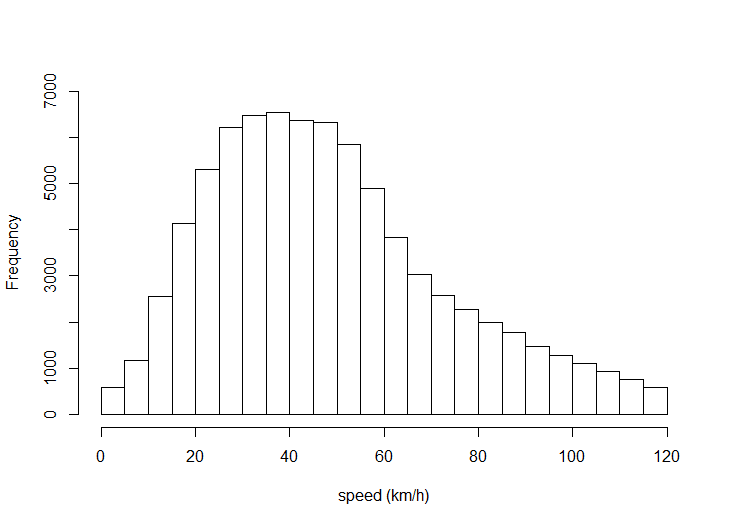
\includegraphics[width=0.7\textwidth]{figures/avg_speed_green_class_matched}}
	{}

\paragraph{Map matching}
Using the MATSim compatible verison of Graphhopper, the GPS points are then matched to the MATSim road network. A measurement sigma of 50m is used to find candidate road segments, and an unlimited distance between consecutive points is allowed. Once the GPS points are matched to road segments, the segment entry and exit times are calculated. This is not performed by Graphhopper. \red{In fact, while relatively state of the art, the Hidden Markov Model approach used by Graphhopper (\cite{vertrbi} doesn't consider speed limits and the respective possible travel times when identifying candidate links for matching.} 

\paragraph{Link entry and exit time calculation}
The map matching module returns a list of $n$ links and the set of GPS points $P(l)$ matched to each link. The recorded time and location of the first and last GPS point $p_{l}$ - ($p_{l,s}$ and $p_{l,e}$ respectively) on each link $l$ are used to estimate the entry and exit times to the link. 
Start and end links must have at least one GPS point associated with them, while intermediate links maybe have none or more GPS points. 
Each GPS point $p_{l,i}$ is projected onto link l, to mark the distance traveled along the link at certain times as $p'_{l,i}$.

A helper function $time\_between(a,b)$ returns the time needed to travel between projected points and verticies of a link. From $p'_{l,e}$ to the end of a link; or the start of a link to the first projected point on a link $p'_{l,s}$. 
$tt(l)$ gives the time needed to travel a link under free flow conditions, and $time_between(p_{l,e}, p_{l',s}$) gives the time difference between the last and first points on two links respectively.

In MATSim the assumptions hold that an agent starts and ends somewhere on a link. Hence, for the first link, only the exit time needs to be calculated, and respectively the entry time for the last link. Additionally, $entry\_time(l_{j}) = exit\_time(l_{j-1}),  \forall j = 1..n$. As such, the algorithm can be separated into two cases:
\begin{itemize}
	\item \textbf{First Link} For the first link $l_1$, $exit\_time(l_1) = time(p'_{l_1,e}) + time\_between(p'_{l_1,e}, l_1)$
%%%	\item \textbf{Last Link} For the last link $l_n$, $entry\_time(l_n) = exit\_time(l_{n-1}) + time\_between(l_{n-1}, p'_{l_n,s})$
	\item \textbf{Other Links} \\
		$entry\_time(l_{j}) = exit\_time(l_{j-1}) $ \\
		\textbf{if} $P(l_j) = \emptyset$ \textbf{then} $exit\_time(l_j) = entry\_time(l_j) + 
										\frac{length(l_j) \cdot time\_between(p'_{l_{j-1},e}, p'_{l_{j+1},s})}{distance(p'_{l_{j-1},e}, p'_{l_{j+1},s})} $ \\
		\textbf{else}  $exit\_time(l_j) = entry\_time(l_j) + time\_between(l_{j}, p'_{l_j,e}) + \frac{time\_between(p'_{l_j,e}, l_{j}) \cdot time\_between(p'_{l_j,e}, p'_{l_{j+1},s})} 
					{time\_between(p'_{l_j,e}, l_{j}) + time\_between(l_{j+1},p'_{l_{j+1},s})}   $ \\
\end{itemize}

\paragraph{Conversion to MATSim events} 
The sequence of links with entry and exit times are then converted to valid MATSim events and grouped by person and date.

\paragraph{Imputation of externalities on MATSim events}
To impute the externalities of each trip leg, The events are processed using a MATSim framework set up with two additional modules. The first, developed by \citet{kaddoura} calculates the pollutant amounts inccured on each link, based on the observed travel speed. Values and emissions factors are taken from the HBEFA database, version 3.2. Average speeds on each link are capped at the link freespeed. The road types for assigning emissions factors are taken from OSM. Each driver is assigned a medium sized vehicle with a 4 cylinder EURO-4 compliant petrol engine. It was not possible at this stage to represent the actual owned vehicles of the study participants.

For congestion, the caused delays per link are imputed from the average hourly values calculated section \ref{avgvalues}. The time lost per link is calculated from the difference between the link travel time and travel time under free flow conditions in the MATSim scenario. From here is it straight forward to determine the total generated pollution and caused and experienced delay per trip leg.

\section{Results}
%% i.e. validation against swiss norms
\subsection{Validation}
%%Chris
To validate the externality values estimated using MATSim, the produced outputs are analyzed both temporally and spatially to check for plausibility and then compared with estimates from previous Swiss external cost reports.

\subsubsection{Emissions}
Emissions values can be estimated with MATSim directly from the processed GPS traces and therefore do not explicitely require a calibrated MATSim scenario for Switzerland.
Nevertheless, in order to validate our estimations, emission values are first calculated using a 10\% MATSim scenario for Switzerland.
To comply with new vehicle registration statistics according to \citet{autoschweiz2010}, \citet{autoschweiz2012} and \citet{energieVerbrauchEffizienzPersonenwagen2015} as well as the vehicle ownership predictions from \citet{foen2010pollutants}, two scenarios where 30\% and 40\% of vehicles are randomly assigned a diesel engine were examined.

The emission values are estimated for each road link in the MATSim network for the following pollutants: CO, total CO$_2$, FC, HC, NMHC, NO$_2$, NO$_x$, PM and SO$_2$.
The values are aggregated into hourly time bins.
These emission estimates are then first analyzed temporally and spatially to assure the plausibility of the output.

When analyzing the temporal evolution of emissions over the course of a typical workday, we would expect it to correlate with typical commuter patterns, i.e. low emissions both in the early morning and late evening and higher emissions during the day, with spikes corresponding to rush-hour periods.
\Cref{fig:hourlyEmissions} shows the typical daily emission of each pollutant per hourly time bin estimated from the MATSim scenario, for both the 30\% and 40\% diesel engine ownership scenarios.
Note that only total CO$_2$ and FC are shown, as the emissions values for the other pollutants are negligeable in comparison.
As expected, two distinct peaks corresponding to morning and evening rush-hour can be observed, while the early morning and late-night values are near zero and the midday values lie somewhere in between.

\createfigure%
{Hourly emissions values for Switzerland}%
{Hourly emissions values for Switzerland. Only total CO$_2$ and FC emissions are shown, as the values for the other pollutants are negligeable in comparison.}%
{\label{fig:hourlyEmissions}}%
{%
  \createsubfigure%
  {30\% diesel vehicles}%
  {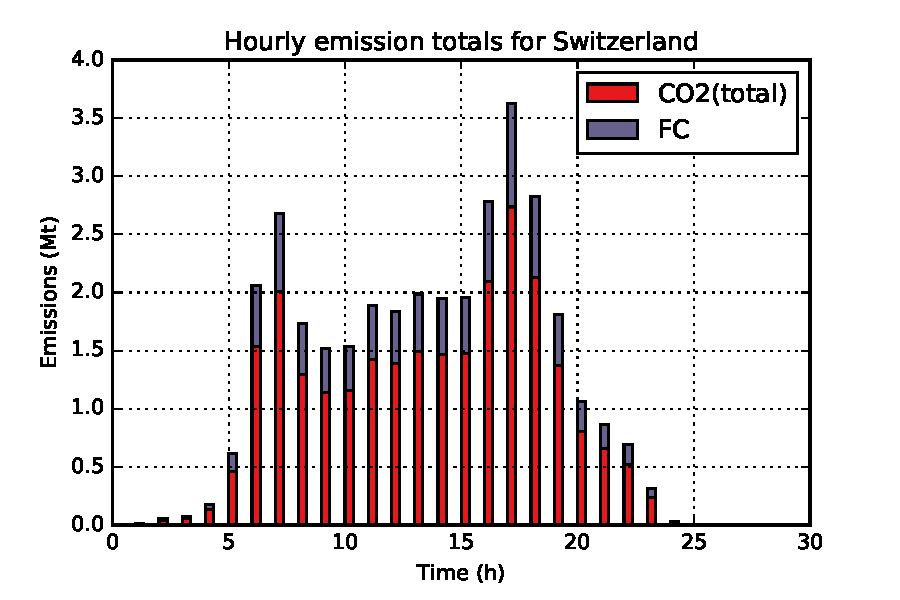
\includegraphics[width=0.49\textwidth,
angle=0]{figures/hourly_emissions_30pct_diesel.pdf}}%
  {\label{fig:hourlyEmissions-30pctDiesel}}%
  {}%
  \createsubfigure%
  {40\% diesel vehicles}%
  {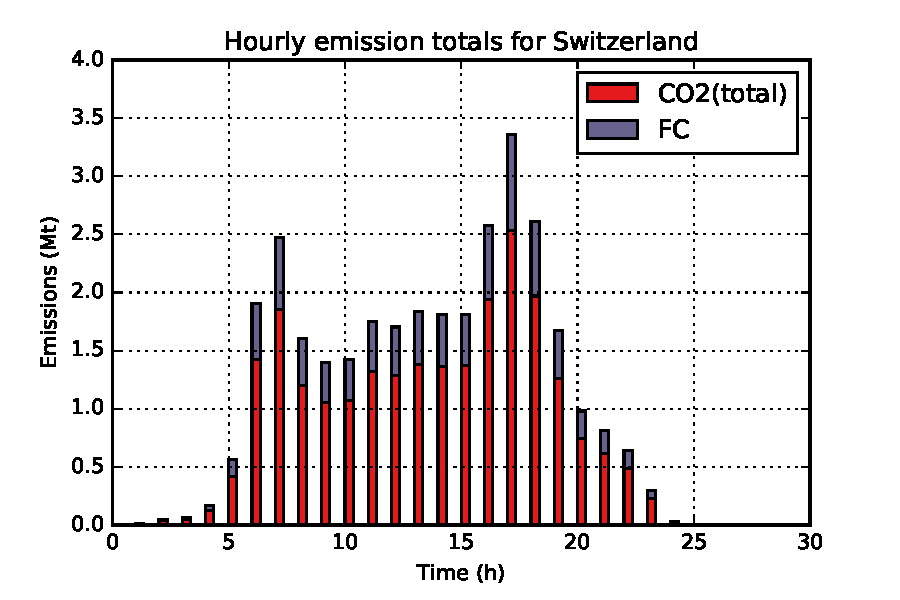
\includegraphics[width=0.49\textwidth,
angle=0]{figures/hourly_emissions_40pct_diesel.pdf}}%
  {}%
}%
{}

The spatial analysis of emissions is expected to show higher emissions in and around larger cities and within highly populated cantons, where more people live and therefore more commutes are observed.
\Cref{fig:spatialEmissions} shows the spatial distribution of the total daily emissions over all of Switzerland with 40\% diesel engine ownership.
The heatmap is generated by summing the total emissions with a 10 km radius around each point.
Indeed, it can be seen that total emission values are higher in the main metropolitan areas (Zurich, Geneva, Basel, Bern, Lausanne, Lucerne, St-Gallen) than in rural areas within e.g. Graub\"unden, Valais, Schwyz or Appenzell.
Higher emissions also tend to coincide with the presence of motorways.

\createfigure%
{Spatial distribution of total emissions in Switzerland with 40\% diesel engines}%
{Spatial distribution of total emissions in Switzerland with 40\% diesel engines}%
{\label{fig:spatialEmissions}}%
{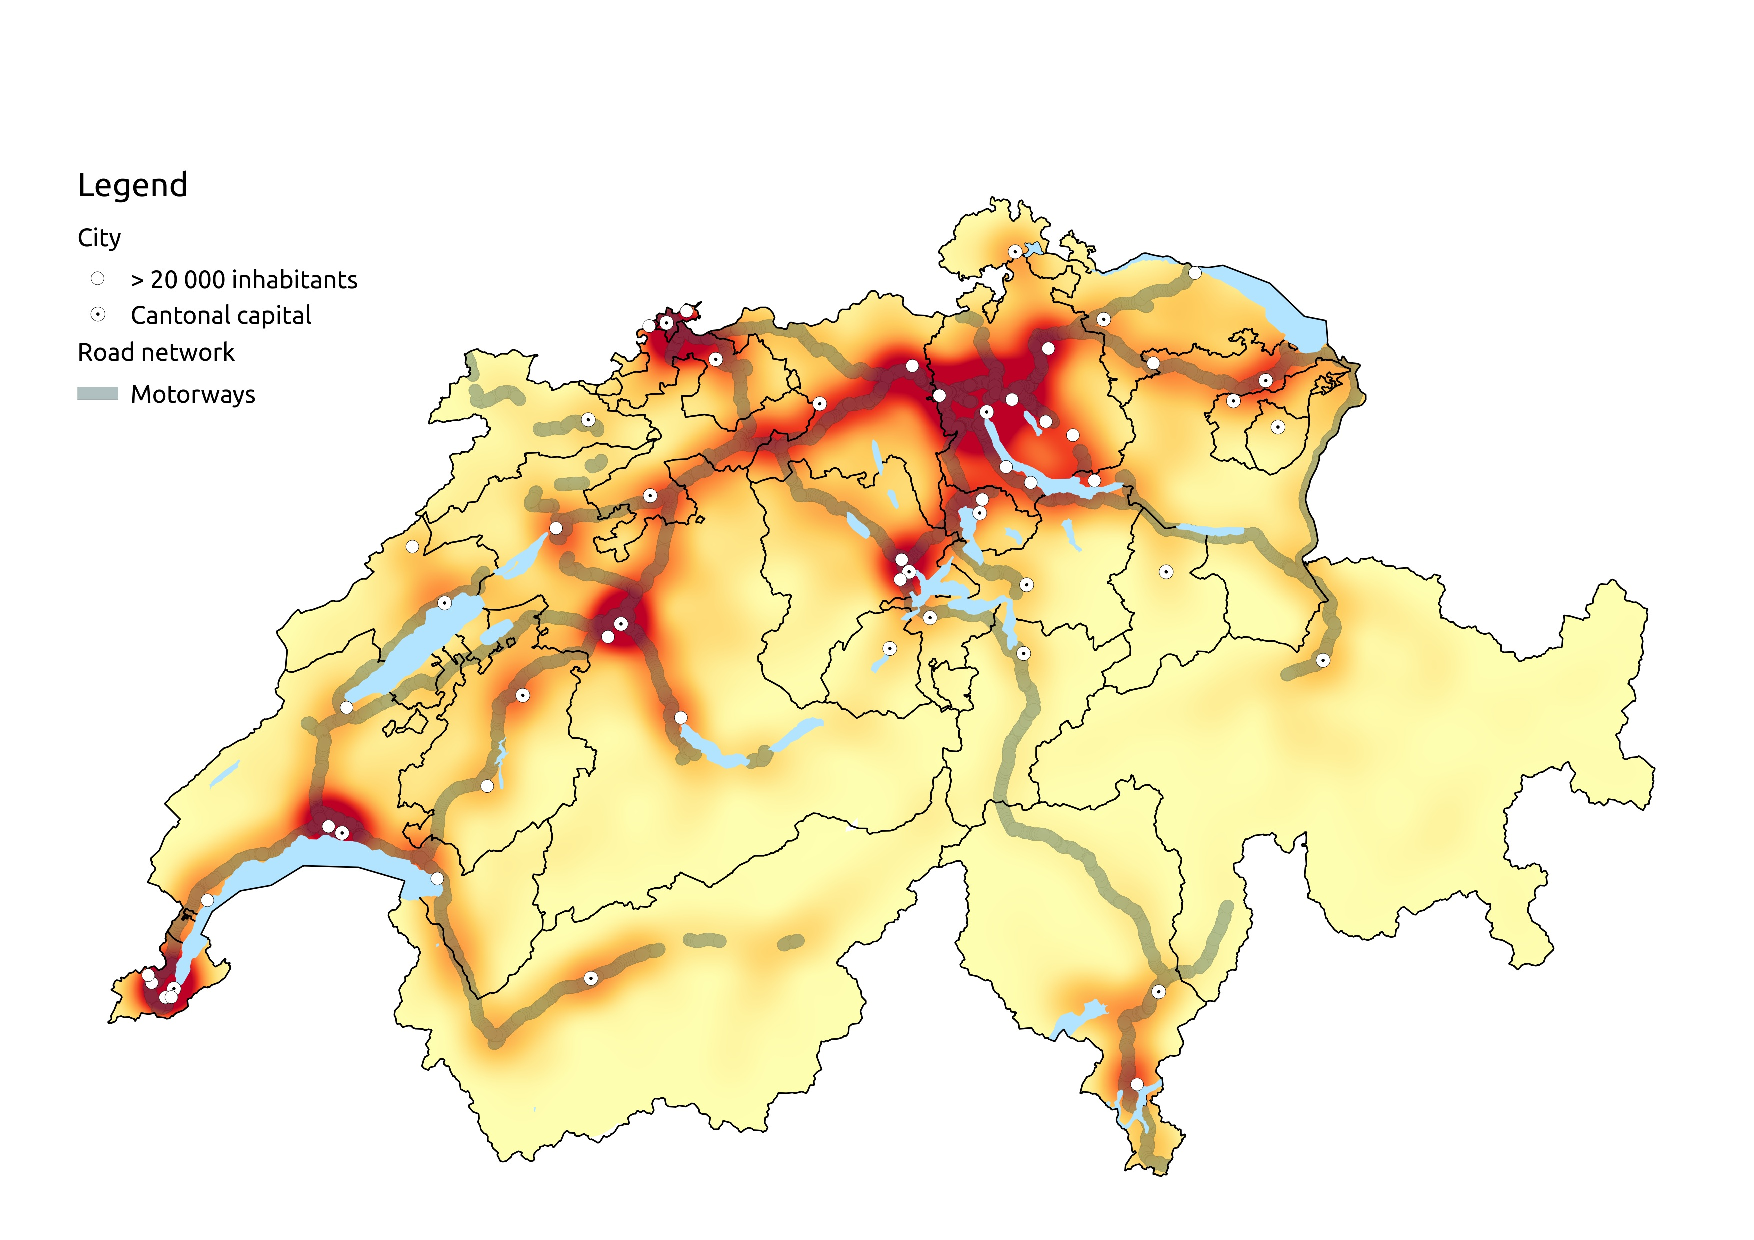
\includegraphics[width=1.0\textwidth, angle=0]{figures/total_emissions_heatmap.pdf}}%
{}

The MATSim computed emissions values are then compared to those estimated by \citet{foen2010pollutants} for 2015.
Since MATSim simulates a single typical workday for 10\% of the entire Swiss population, our values need to be scaled in order to be comparable.
The emissions values are thus multiplied by 10 to account for the population sampling, then by 365 days and finally by an additional scale factor such that the total traveled distance matches the one reported by \citet{foen2010pollutants} for 2015.
\Cref{tab:emissionValueMatsimFoenComparison} shows the total estimated emissions values for both MATSim scenarios and \citet{foen2010pollutants} and \Cref{fig:emissionValueMatsimFoenComparison} plots the percent deviation of the MATSim estimates from the reported 2015 estimates.
The total emission values for all pollutants except PM are within 40\% of the reported values; the values for NO\textsubscript{x}, NO\textsubscript{2} and PM increase with an increase in the diesel engine ownership share.
These deviations are possibly due to the fact that emissions factors depend on the exact type of petrol or diesel engine.
Indeed, in the MATSim model, only one type of petrol and diesel engine is considered, whereas in reality, these are further subdivided into specific subtypes with different emission standards.
Further calibration of the vehicle engine types to the appropriate subtypes could possibly lead to a better fit in emissions values.
Nevertheless, the estimed values coincide with the previously reported values, thereby demonstrating that MATSim provides a reliable means of estimating emission values for pollutants.


\createtable%
{MATSim and FOEN estimated emission value comparison}%
{MATSim and FOEN estimated emission value comparison}%
{\label{tab:emissionValueMatsimFoenComparison}}%
{%
  \begin{tabular}[c]{lrrrrr}
    \toprule
    \multirow{3}{*}{Pollutant} & \multirow{3}{*}{FOEN} & \multicolumn{4}{c}{MATSim} \\ 
    & & \multicolumn{2}{c}{30\% diesel} & \multicolumn{2}{c}{40\% diesel}\\
    & t/a & t/a & \% & t/a & \% \\
    \midrule
	CO\textsubscript{2} (total)  &  10 687 911 &    12 580 738 &	17.71 &	   11 651 538 &		 9.02 \\
	FC         					 &           0 &     4 130 052 &	  --- &     3 823 821 &		  --- \\
	CO         					 &      67 424 &        89 789 &	33.17 &        78 879 &		16.99 \\
	NO\textsubscript{x}     	 &      16 496 &        16 635 &	 0.85 &        20 530 &		24.46 \\
	HC       					 &       9 546 &        10 014 &	 4.90 &         8 952 &		-6.23 \\
	NMHC 					     &       9 037 &         9 467 &	 4.76 &         8 473 &		-6.24 \\
	NO\textsubscript{2}        	 &       4 127 &         4 175 &	 1.15 &         5 441 &		31.83 \\
	PM        					 &         418 &           621 &	48.46 &           764 &		82.67 \\
	SO\textsubscript{2}        	 &          59 &            61 &	 3.06 &            56 &		-4.28 \\
    \bottomrule
  \end{tabular}
}%
{}

\createfigure%
{MATSim and FOEN estimated emission value comparison}%
{MATSim and FOEN estimated emission value comparison}%
{\label{fig:emissionValueMatsimFoenComparison}}%
{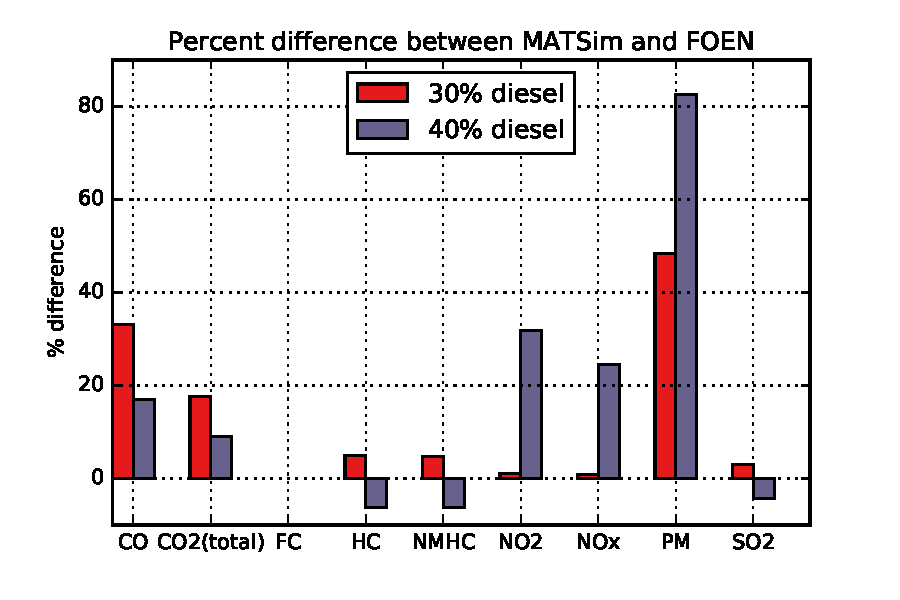
\includegraphics[width=1.0\textwidth, angle=0]{figures/percent_differences.pdf}}%
{}

\subsubsection{Congestion}

Contrary to emissions, congestion and delays caused and experienced cannot directly be estimated from GPS traces alone, since information on how many other drivers were present on the road at that given moment is lacking.
It is precisely for this reason that MATSim is used to estimate congestion throughout a typical workday.
Therefore, it is crucial that the estimated aggregate congestion values are consistent with other previous estimates.
As before, these values are calculated using a 10\% MATSim scenario for Switzerland and are aggregated into hourly time bins per road link.
These estimates are again first analyzed temporally and spatially to assure the plausibility of the output before being compared to the values from \citet{mkinfras2016staukosten}.

The typical total caused and experienced delays pattern per hourly time bin estimated from the MATSim scenario is shown in \Cref{fig:hourlyDelays}.
As was the case for emissions, total delays also expectedly coincide with typical commuter patterns, with fewer delays the early morning and at night, two distinct peaks corresponding to morning and evening rush-hour and midrange values at midday.
One notices in \Cref{fig:hourlyDelays} that there are higher caused delays than experienced delays at the start of the peaks whereas the opposite is true towards the end of the peaks, a manifestation of the fact that delays first need to be caused before they can be experienced.
Nonetheless, the total duration of both caused and experienced delays are equal and sum up to just under 250 000 hours.


\createfigure%
{Hourly total caused and experienced delays for Switzerland}%
{Hourly total caused and experienced delays for Switzerland}%
{\label{fig:hourlyDelays}}%
{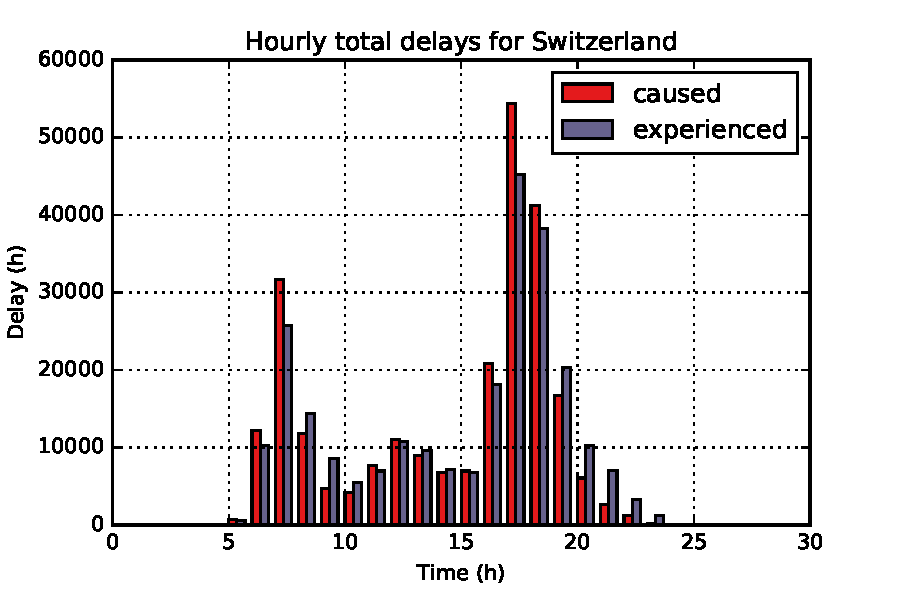
\includegraphics[width=0.8\textwidth,
angle=0]{figures/hourly_delays.pdf}}%
{}

\Cref{fig:spatialDelays} shows the spatial distribution of the total daily experienced delays over entire Switzerland.
The heatmap is generated by summing the total experienced delays with a 1 km radius around each point.
Following an anogolous reasoning as for emissions, longer delay times are observed in and around larger cities and within highly populated cantons, where more people live and commute to.

\createfigure%
{Spatial distribution of total experienced delays in Switzerland}%
{Spatial distribution of total experienced delays in Switzerland}%
{\label{fig:spatialDelays}}%
{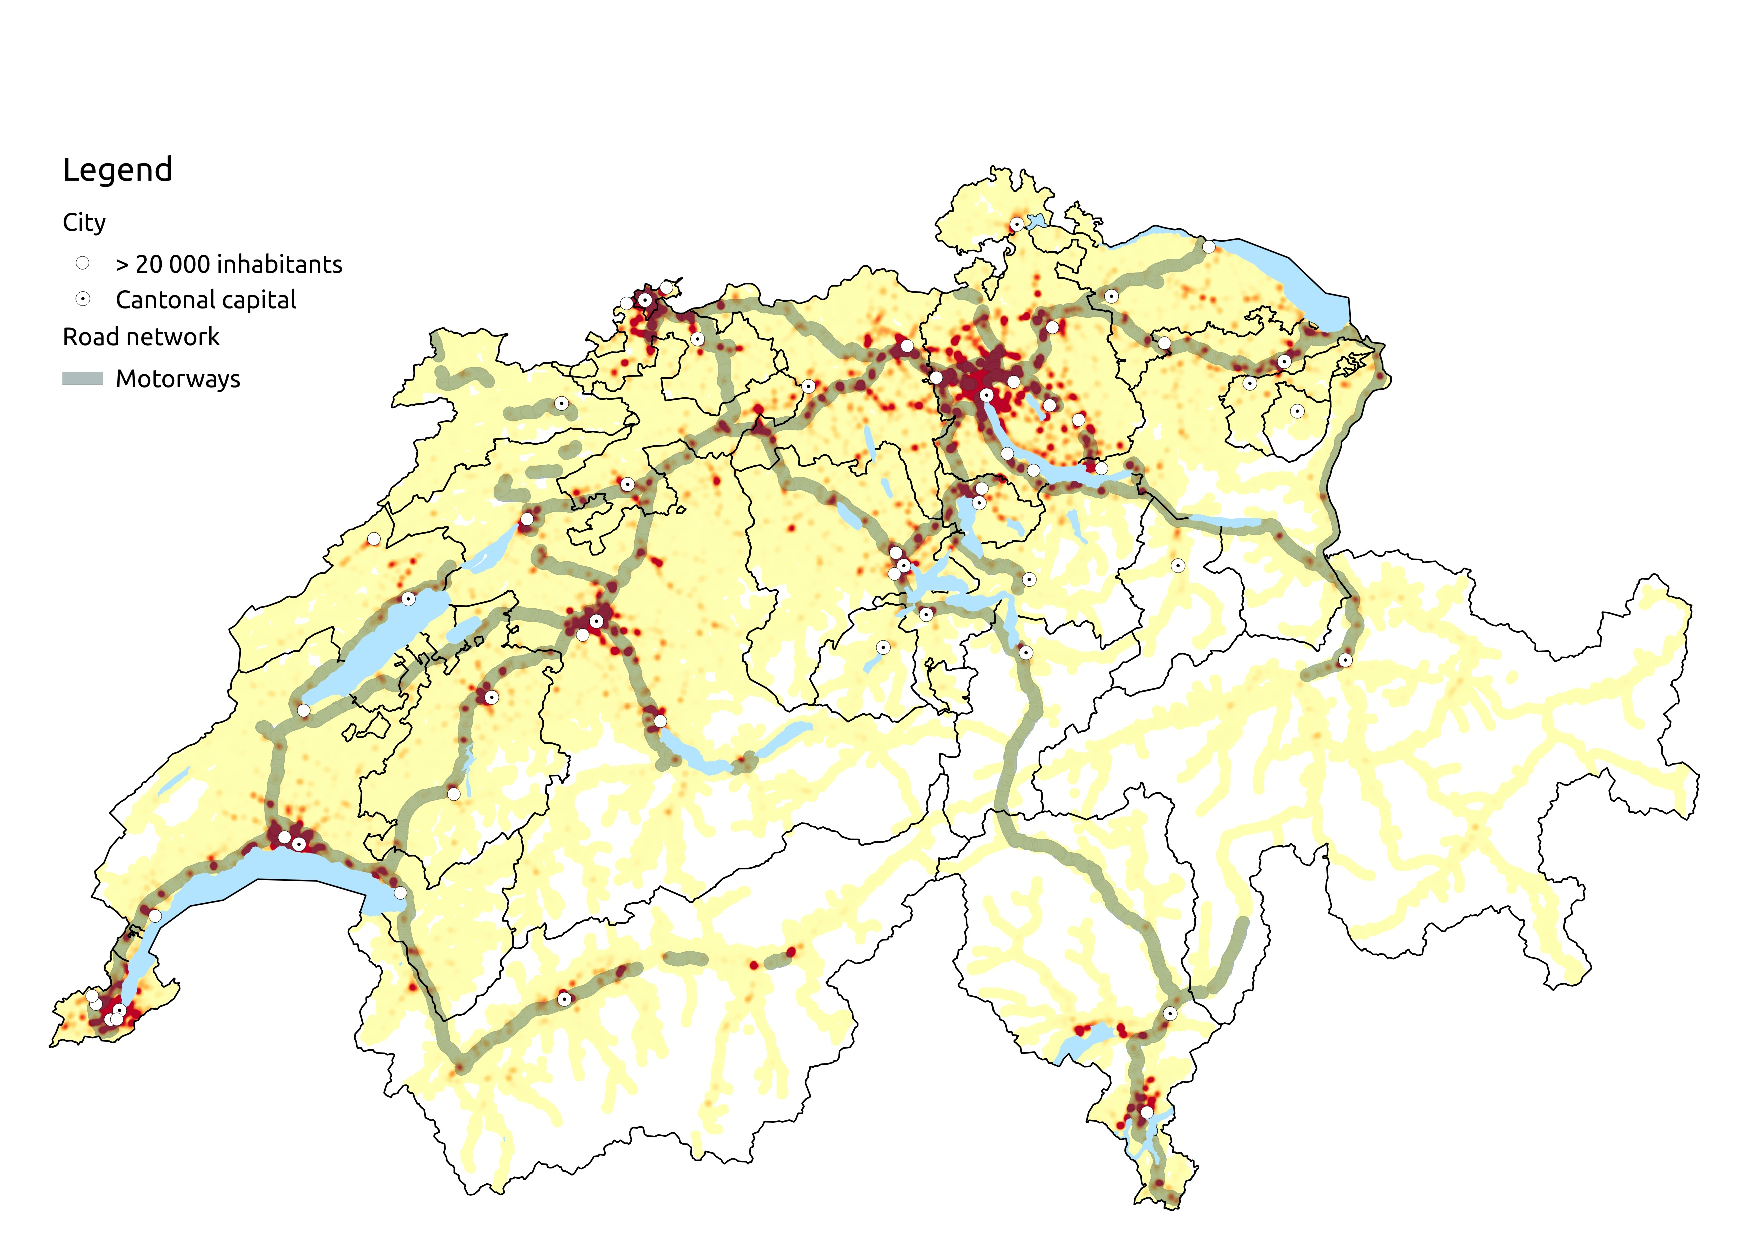
\includegraphics[width=1.0\textwidth, angle=0]{figures/total_delays_heatmap.pdf}}%
{}

The MATSim computed delay values are then compared to those calculated by \citet{mkinfras2016staukosten}.
The same scaling operations are performed as in the case of emissions: multiplication by 10 to account for the population sampling, then by 365 days and finally by an additional scale factor such that the total traveled distance matches the one reported by \citet{mkinfras2016staukosten} for 2014.
The values are reported in \Cref{tab:delayValueComparison}.


\createtable%
{MATSim and Infras / MK Consulting congestion comparison}%
{MATSim and Infras / MK Consulting congestion comparison}%
{\label{tab:delayValueComparison}}%
{%
  \begin{tabular}[c]{lrrr}
    \toprule
    Road type & MK/Infras (Mveh-h/a) & MATSim (Mveh-h/a) & \%  \\ 
    \midrule
    Motorway      & 16.62 &    8.33 &  -49.89 \\
    Non-motorway  & 11.23 &   95.00 &  745.98 \\
    Total &         27.85 &  103.33 &  271.03 \\
    \bottomrule
  \end{tabular}
}%
{}

The total vehicle hour delay per year values are estimated to be much higher in MATSim than in \citet{mkinfras2016staukosten}.
However, the authors do indeed state that they have taken an "at-least" approach in estimating delays and that the values for non-motorway segments are highly underestimated.
On the other hand, our model only simulates passengers vehicles.
Therefore, it neither accounts for the effects of the interaction of cars with trucks on motorways nor does it captures extraordinary circumstances such as accidents and holiday traffic which could increase the vehicle hours of delay.
A combination of these effects could be the underlying cause of the deviation between the estimates and should be further investigated.


\subsection{Green Class Emission Reductions}
A core component of the Green Class pilot project was the availability of an electric car to subscribers. These cars were covered by renewable energy certificates, negating the need to consider the energy generation makeup in calculating the emissions reductions. For the analysis, it is assumed that for trips performed with an electric vehicle, the driving style, route choice and trip timing is independent of the choice of vehicle. Additionally, the possibility that the availability of electric vehicles generated mode shifts away from other modes (i.e. train travel, cycling or car sharing) is excluded. 
The effects of having an additional vehicle in multi-car households are also excluded. 

\createtable%
{Reduction in emissions due to the availability of an electric vehicle}%
{Reduction in emissions due to the availability of an electric vehicle}%
{\label{tab:reduction_summary}}%
{%
\begin{tabular}{rrrr}
  \hline
 & Car & Ecar & Reduction (\%) \\ 
  \hline
CO (kg) & 45.51 & 37.26 & 45.02 \\ 
  CO\textsubscript{2} (T) & 11.32 & 8.97 & 44.20 \\ 
  FC (T) & 3.60 & 2.85 & 44.20 \\ 
  HC (kg) & 4.53 & 3.68 & 44.80 \\ 
  NMHC (kg) & 4.27 & 3.46 & 44.80 \\ 
  NO\textsubscript{x} (kg) & 24.18 & 19.34 & 44.43 \\ 
  NO\textsubscript{2} (kg) & 4.12 & 3.28 & 44.37 \\ 
  PM (kg) & 1.22 & 0.97 & 44.29 \\ 
  SO\textsubscript{2} (kg) & 0.06 & 0.05 & 44.20 \\ 
   \hline
\end{tabular}
}%
{}

\Cref{tab:reduction_summary} presents the reduction of various emissions over the course of the program due to the availability of the E-car. 
A clear immediate reduction in daily CO\textsubscript{2} emissions is observed in \Cref{fig:green-class-reduction}. 
Overall, a reduction of 30\% can be observed with respect to the pre-Ecar period. 
There are however some noticeable outliers, particularly April 1\textsuperscript{st}, 2017. 
During the course of the pilot program, subscribers had unrestricted access to both their personal vehicle and the provided electric vehicle. 
As such, on days where many subscribers choose to use their personal vehicles, emissions will naturally be nearer to the pre-program levels. 
A particular reason for such a choice would be public holidays where many subscribers are likely to want to travel further than what the range of the electric vehicle permits.

\createfigure%
{Percentage of pre-electric vehicle CO\textsubscript{2} produced per day. EV's were provided on January 16, 2017. }%
{Percentage of pre-electric vehicle CO\textsubscript{2} produced per day. EV's were provided on January 16, 2017. }%
{\label{fig:green-class-reduction}}%
{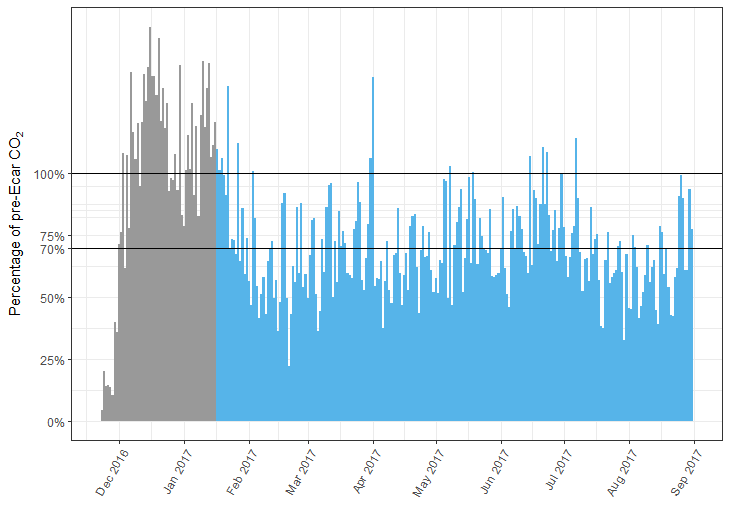
\includegraphics[width=1.0\textwidth, angle=0]{figures/green_class_pollutant_reductions_daily}}%
{}

The 139 subscribers were not representative of the general population, due to the high cost (12,200 CHF) and selective nature of the pilot program.
Nevertheless, these results demonstrate the environmental benefit of having an electric vehicle, and that persons with access to both will significantly reduce their emissions by using the electric vehicle.

%%%%%%TODO: add a comparison of congestion experienced vs congsetion caused for Green Class drivers
\section{Conclusion}
%%Joe
This paper presented a methodology for imputing the externalities on GPS traces using the MATSim framework. 
The 2015 MATSim Switzerland scenario was used to provide hourly aggregate estimates for incurred and caused congestion, and pollutant emission factors were taken from the Handbook for Emission Factor Analysis (HBEFA). 
The suitability of the MATSim scenario for this purpose was evaulated by validating the Switzerland wide externaties against published offical values. 
The agent-based aspect of MATSim allows for much finer calculation of externalities by taking into account the heterogenity in both the population and travel behaviour. 
The validation indicated that the 2015 scenario is mostly suitable for such purposes with some caveats. 
Firstly, the emissions results are highly dependent on the make-up of the national car fleet. 
As such further work will incorportate a car ownership model for Switzerland into the scenario.
Secondly, the total delay hours in the scenario are lower than the offical numbers for motorways, but higher for other roads. 
While the errors are most likely introducted from simplifications on both sides, more work needs to be done to identify the sources of these discrepancies.
The analysis of the SBB Green Class project with the proposed methodology illustrate the environmental benefits of electric vehicles in mobility schemes, even when convential alternatives are still available. Ongoing work will explore the experienced and caused congestion of subscribers, and identify how such information can be communicated to respondents to influence thier travel behaviour. 

\section{Aknowledgement}
This research was supported by the Swiss National Research Foundation and the Swiss Compentency Center for Energy Research.


%%%%%%%%%%%%%%%%%%%%%%%%%%%%%%%%%%%%%%%%%%%%%%%%%%%%%%%%%%%%%%%%%%%%%%
%% Bibliography
%%   Leave this as is, and add you own entries to my.bib
%%   Many references are already defined in _latexfiles/bibs/all-eng.bib
%%   Refer to the BibTeX/LaTeX tutorial for adding new entries
%%   to the IVT BibTeX database
\bibliography{\mypath bibs/all-eng,my}
%%%%%%%%%%%%%%%%%%%%%%%%%%%%%%%%%%%%%%%%%%%%%%%%%%%%%%%%%%%%%%%%%%%%%%

%%%%%%%%%%%%%%%%%%%%%%%%%%%%%%%%%%%%%%%%%%%%%%%%%%%%%%%%%%%%%%%%%%%%%%
%% Appendices
%%   Usually they would start on a separate page
%%%%%%%%%%%%%%%%%%%%%%%%%%%%%%%%%%%%%%%%%%%%%%%%%%%%%%%%%%%%%%%%%%%%%%

\clearpage

\end{document}

%%%%%%%%%%%%%%%%%%%%%%%%%%%%%%%%%%%%%%%%%%%%%%%%%%%%%%%%%%%%%%%%%%%%%%
%%%%%%%%%%%%%%%%%%%%%%%%%%%%%%%%%%%%%%%%%%%%%%%%%%%%%%%%%%%%%%%%%%%%%%
%%
%% END OF DOCUMENT
%%
%%%%%%%%%%%%%%%%%%%%%%%%%%%%%%%%%%%%%%%%%%%%%%%%%%%%%%%%%%%%%%%%%%%%%%
%%%%%%%%%%%%%%%%%%%%%%%%%%%%%%%%%%%%%%%%%%%%%%%%%%%%%%%%%%%%%%%%%%%%%%

%%%%%%%%%%%%%%%%%%%%%%%%%%%%%%%%%%%%%%%%%%%%%%%%%%%%%%%%%%%%%%%%%%%%%%
%% Editor specific keywords:
%%   This is not part of you paper, but sometimes it is used
%%   for additional features of TeX Editors.
%%
%% WinEdt:
%%   to get the bibliography list
%GATHER{./_bibs/all-eng.bib}
